\documentclass[12pt]{article} 
\usepackage{fullpage} 
\usepackage[affil-it]{authblk} 
\newcommand{\tab}{\hspace*{2em}}
\usepackage{graphicx} 
\usepackage{caption}
\usepackage{subcaption}
\graphicspath{ {.} } 
\usepackage{float} 
\usepackage{url} 
\usepackage{mhchem}
\usepackage{siunitx}
\usepackage{amsmath}
\usepackage{xfrac}

\begin{document} 

\title{Comparing CENNS detector simulations of Geant4 and MCNP} 

\author[1]{Jan P. Adam} 
\author[2]{Kate Scholberg} 
\affil[1]{Technische Universit\"at Dortmund, Fakult\"at Physik, Dortmund, Germany} 
\affil[2]{Duke University, Department of Physics, Durham, NC 27705} 
\date{October 27, 2014} 

\maketitle
\begin{abstract}
The Spallation Neutron Source (SNS) at Oak Ridge National Laboratory is also a neutrino source. The Duke Neutrino Group has built a detector prototype to observe coherent elastic neutrino-nucleus scattering (CENNS), a process that has been predicted but never observed so far. Beforehand, the detector was simulated with the MCNP-Polimi framework and the goal of this paper is to reproduce the results with Geant4.
\end{abstract}
\newpage

\section{Simulation setup}

The Geant4 simulation toolkit was used to reproduce the results of \cite{MCNP}. The detector setup can be seen in figure \ref{fig:detector}. The detector's core consists of a lead cube (\SI{50}{cm} edge-length) with 4 holes that hold one EJ-301 scintillator, each. These are frustums of a cone and are made of pure liquid EJ-301 (\cf{C_8H_{10}}). The sides and the bottom of the lead cube are covered with a \SI{1}{cm} thick layer of EJ-200 a solid plastic scintillator (\cf{C_{10}H_{11}}). Above the lead cube is a gap of \SI{21}{cm} followed by an Al-7075 plate with a thickness of \SI{2}{cm}. This plate shall reduce signals of cosmic rays in the real detector. The whole setup is enclosed by a \SI{1}{m^3} water cube.

\begin{figure}[htbp]
	\centering
	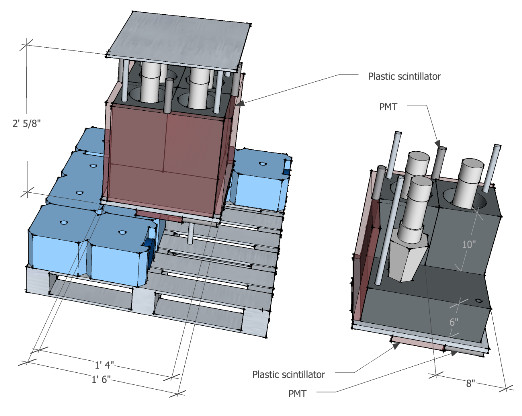
\includegraphics[width=0.7\textwidth]{./pics/Det2.jpg}
	\caption{Layout of the detector. PMTs on top of the scintillators and rods to stabilize the setup were not simulated. The water bricks were replaced by a wall of pure water (no gaps or plastic inside) to speed up the simulation. }
	\label{fig:detector}
\end{figure}

Neutrons are being generated only inside the lead at a random position with a random direction.
If a particle enters one of the scintillators and deposits energy, that amount will be converted into electron-equivalent energy by using the graph in figure \ref{fig:photonResponse}.
\begin{figure}[htbp]
	\centering
	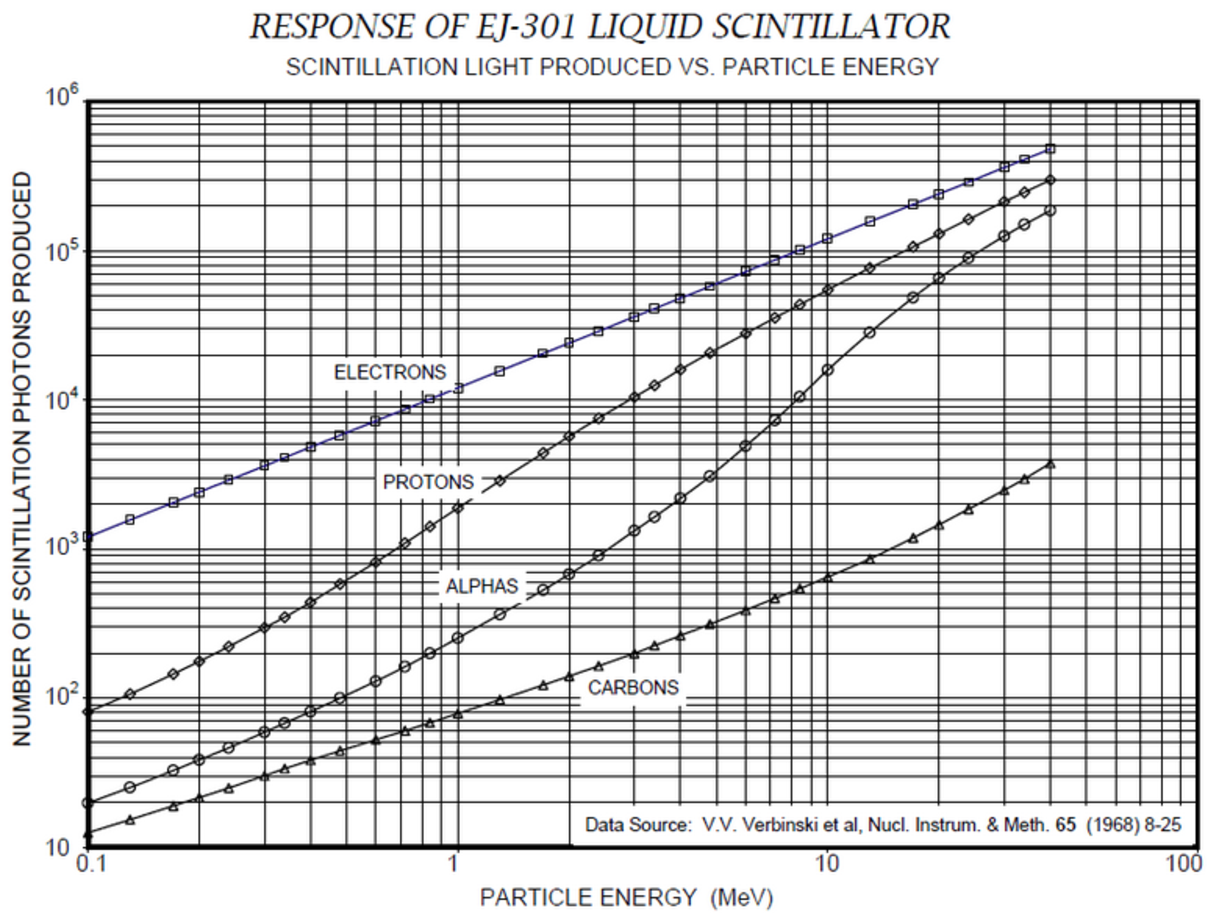
\includegraphics[width=0.81\textwidth]{./pics/scintillatorResponse.pdf}
	\caption{Photon response of the EJ-301 scintillator.}
	\label{fig:photonResponse}
\end{figure}
In addition to the four particles mentioned in figure \ref{fig:photonResponse} there is also a number of $\gamma$, $e^+$ and deuterons that enter the scintillator. Since $e^+$ have the same mass and charge as $e^-$ and $\gamma$ will pair-produce into $e^- + e^+$, both ($\gamma$ and $e^+$) are treated as electrons. Deuterons will approximately emit a number of photons that lies in the middle between $p$ and $\alpha$. 

Also, in approx. 0.5\% of the events the reaction 
\begin{align}
	\ce{n^1_0 + C^{12}_6 \rightarrow C^{13}_6 \rightarrow B^9_4 + \alpha^4_2 } 
\end{align}
can occur. The electron-equivalent energy of the beryllium nucleus will not be calculated because this effect should be negligible.

\section{Results and Discussion}
%
%\subsection{Correct set up} 
%
%First of all, it was necessary to verify that the neutrons were generated in the correct volume. Figure \ref{} and \ref{} show that the particles were generated only inside the lead and not inside the holes which contain the scintillators. Figure \ref{} and \ref{} show that the direction of the neutrons is equally distributed.
%

\subsection{Efficiency}

An event will be marked as "valid" once the energy deposition in a single scintillator exceeds a given threshold in keVee.  Figure \ref{fig:efficiency30} and \ref{fig:efficiency100} show the percentage of how many events were marked as "valid" at a given energy of the primary particle. Two different thresholds \SI{30}{keVee} and \SI{100}{keVee} were used.

 \begin{figure}[H]
 	\begin{subfigure}[t]{0.49\textwidth}
 		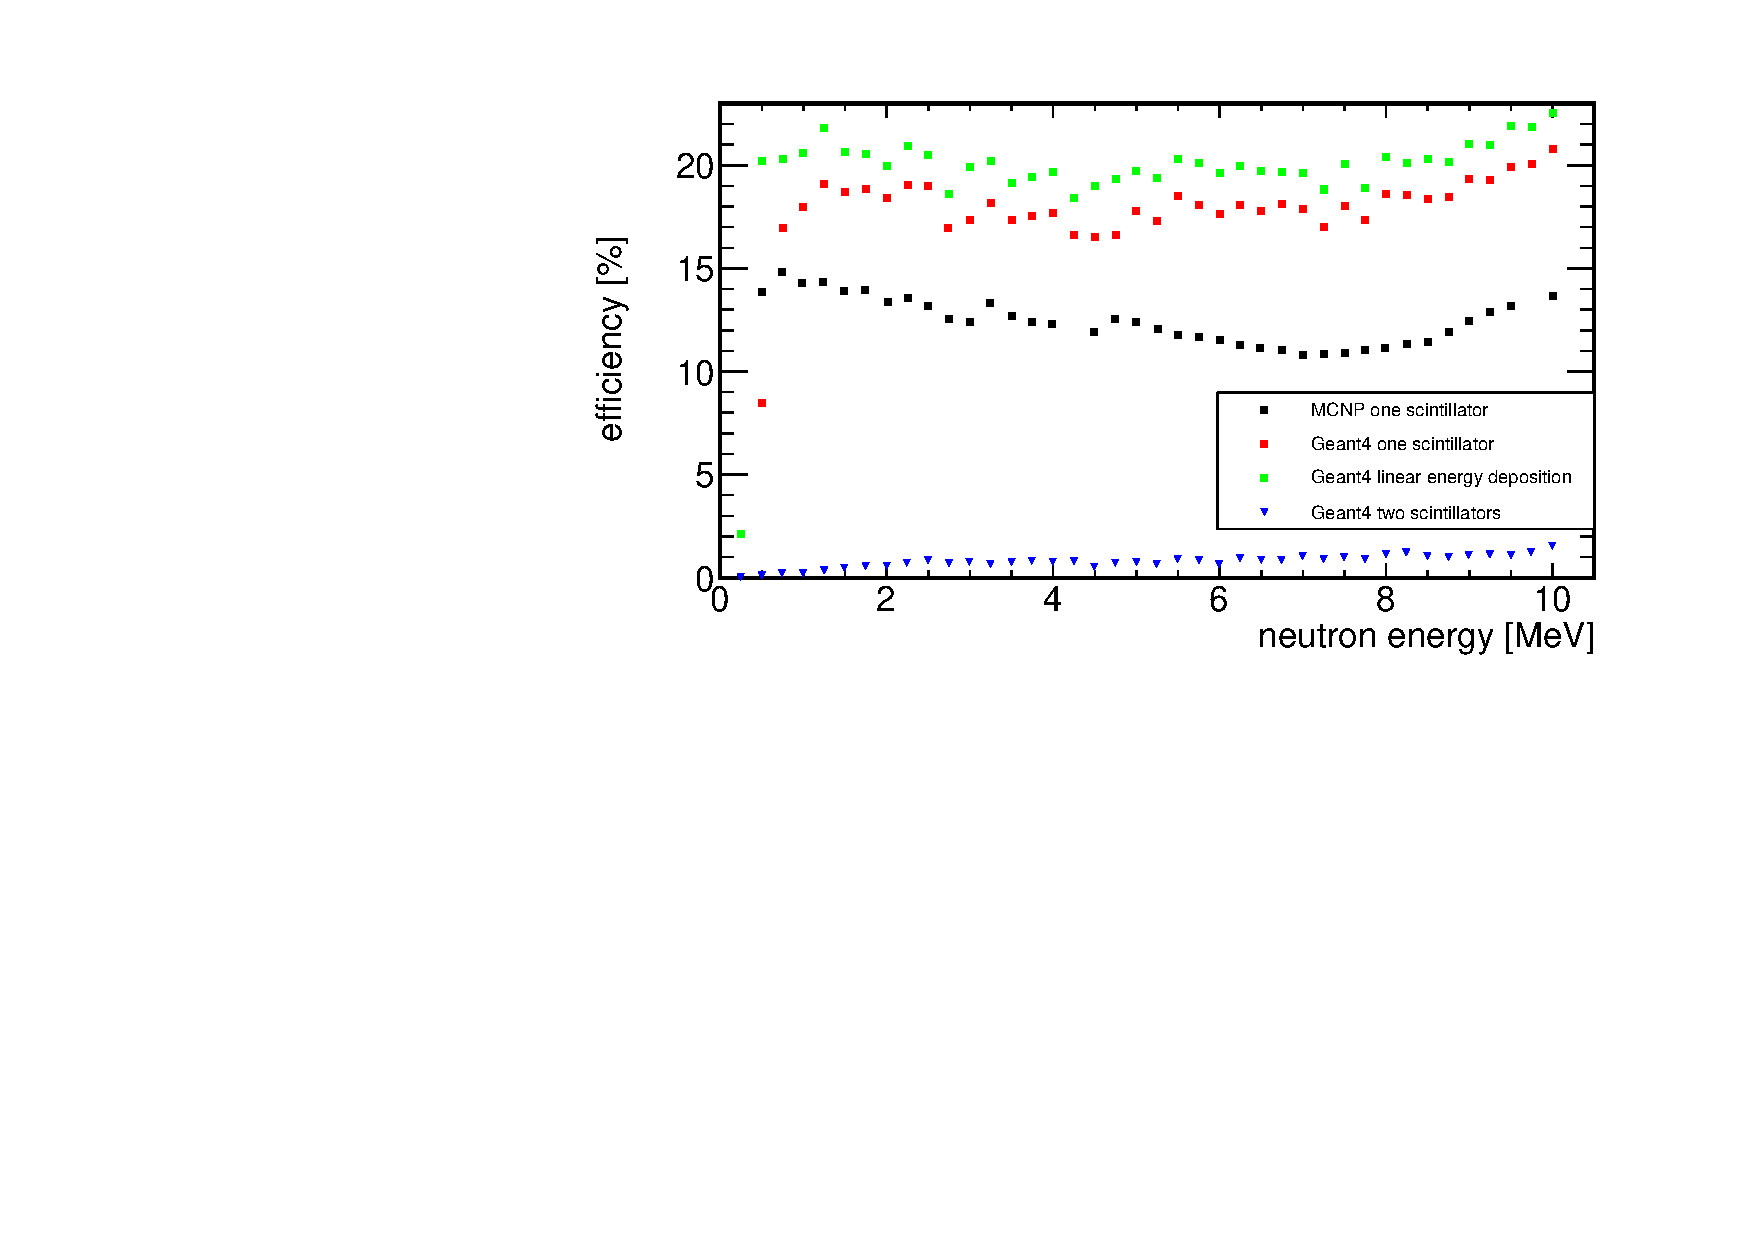
\includegraphics[width=\textwidth]{pics/efficiencyComplete30.pdf}
 		\caption{30 keVee threshold}
 		\label{fig:efficiency30}
 	\end{subfigure}
 	\begin{subfigure}[t]{0.49\textwidth}
 		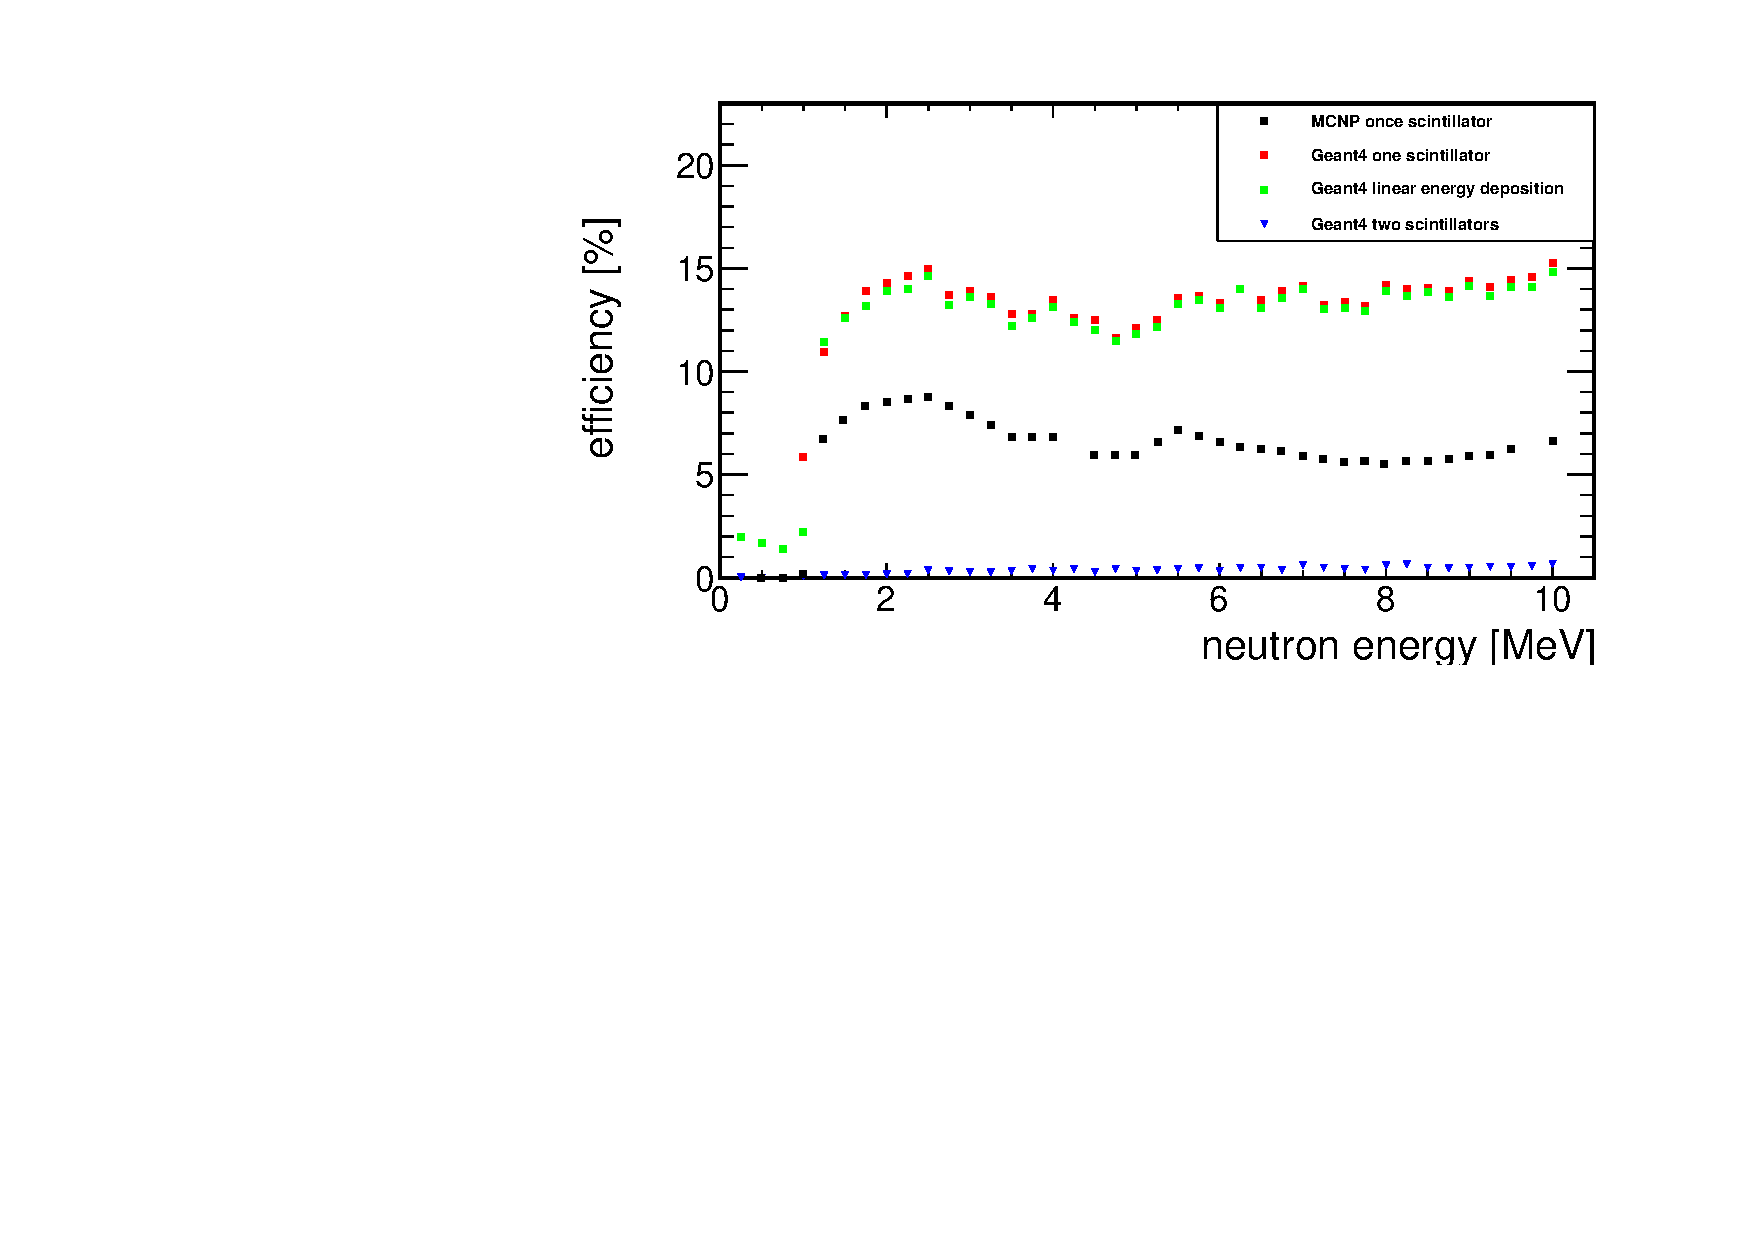
\includegraphics[width=\textwidth]{pics/efficiencyComplete100.pdf}
 		\caption{100 keVee threshold}
 		\label{fig:efficiency100}
 	\end{subfigure}
 	\caption{Percentage of "valid" events for given monochromatic primary particles with a given threshold. MCNP results of "two scintillators" were not included, they varied between 0-1\%.}
 	\label{fig:efficiency}
 \end{figure}
 
 It has to be noted that \label{part:eResponse} the MCNP code did not use figure \ref{fig:photonResponse} to convert the deposited energy to keVee. Instead it was assumed that the scintillator response of a proton is about $\sfrac{1}{10}$\hspace{2pt}th and of a carbon \sfrac{1}{100}\hspace{2pt}th that of an electron. This approximation is valid for low energies but at $\sim\SI{0.7}{MeV}$ the proton response of protons rises. 
 Figures \ref{fig:primaryEnergyMCNP} and \ref{fig:primaryEnergyGeant4} show that most neutrons have energies $>\SI{1}{MeV}$. Therefore the non-linear part might not be negligible.
  \begin{figure}[htbp]
  	  		\centering
  	\begin{subfigure}[t]{0.4\textwidth}
  		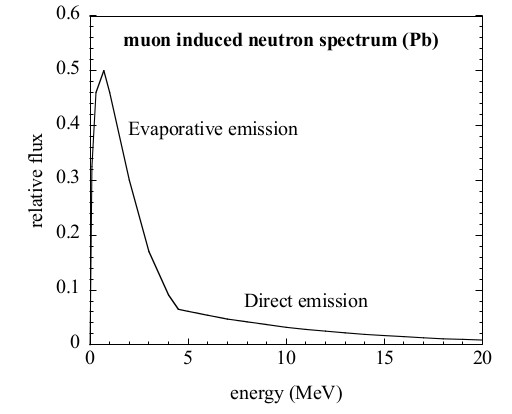
\includegraphics[width=\textwidth]{./pics/primaryEnergy_orig.jpg}
  		\caption{Used for MCNP simulation}
  		\label{fig:primaryEnergyMCNP}
  	\end{subfigure}
  	\begin{subfigure}[t]{0.55\textwidth}
  		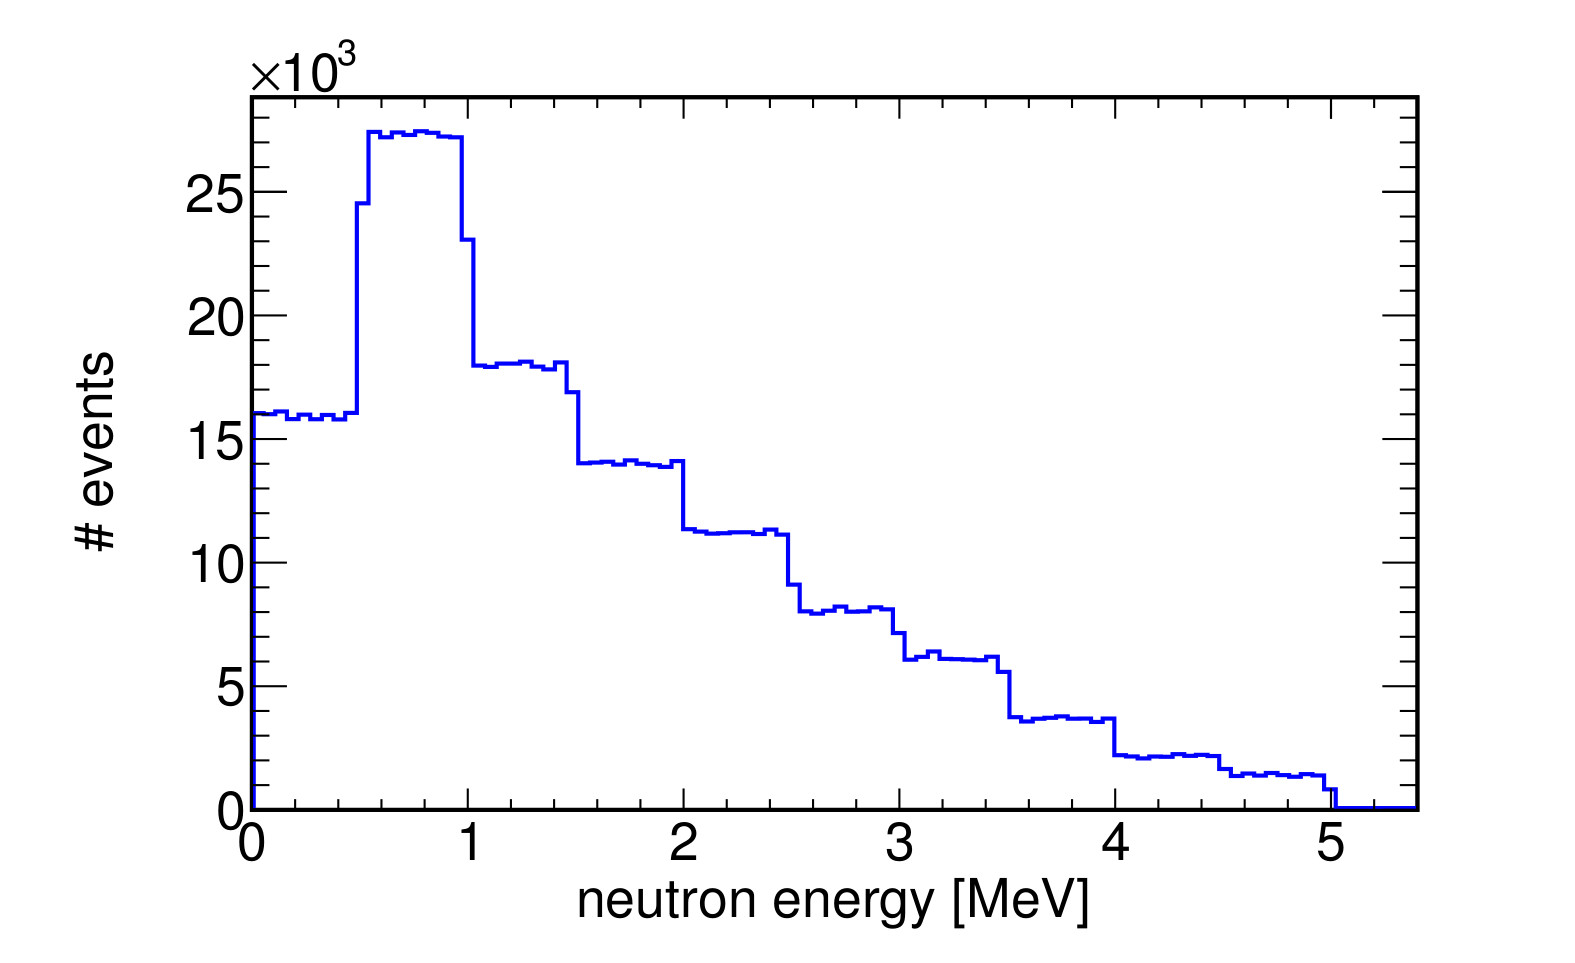
\includegraphics[width=\textwidth]{./pics/primaryEnergy.jpg}
  		\caption{Used for Geant4 simulation}
  		\label{fig:primaryEnergyGeant4}
  	\end{subfigure}
  	\caption{Energy distribution of the primary neutrons. A \SI{5}{MeV} cutoff was used in both programs. To emulate a distribution like  \ref{fig:primaryEnergyMCNP}, 10 data points were read by a digitizer. This results in the sharp edges in \ref{fig:primaryEnergyGeant4}.}
  	\label{fig_primaryEnergies}
  \end{figure}
  
 The efficiency of the Geant4 simulation is about 5\% higher. This might be a result of the different tracking algorithms of Geant4 which will also track secondaries, whereas the MCNP simulation was run in neutron and photon mode only \cite[p.2]{MCNP}. 
 
 Also, the scintillators were simulated as frustums of a cone instead as frustums of a hexagonal pyramid. This increases the cross-sectional area of each scintillator slightly and might result in more valid events.   
 
\subsection{Timing}

Figure \ref{fig:timing30} shows a distribution of the arrival time of the signal. The neutron is being generated at $t=\SI{0}{ns}$ and a signal arrives once the energy deposition one scintillator exceeds a given threshold (\SI{30}{keVee}) for the first time.
 \begin{figure}[H]
 	     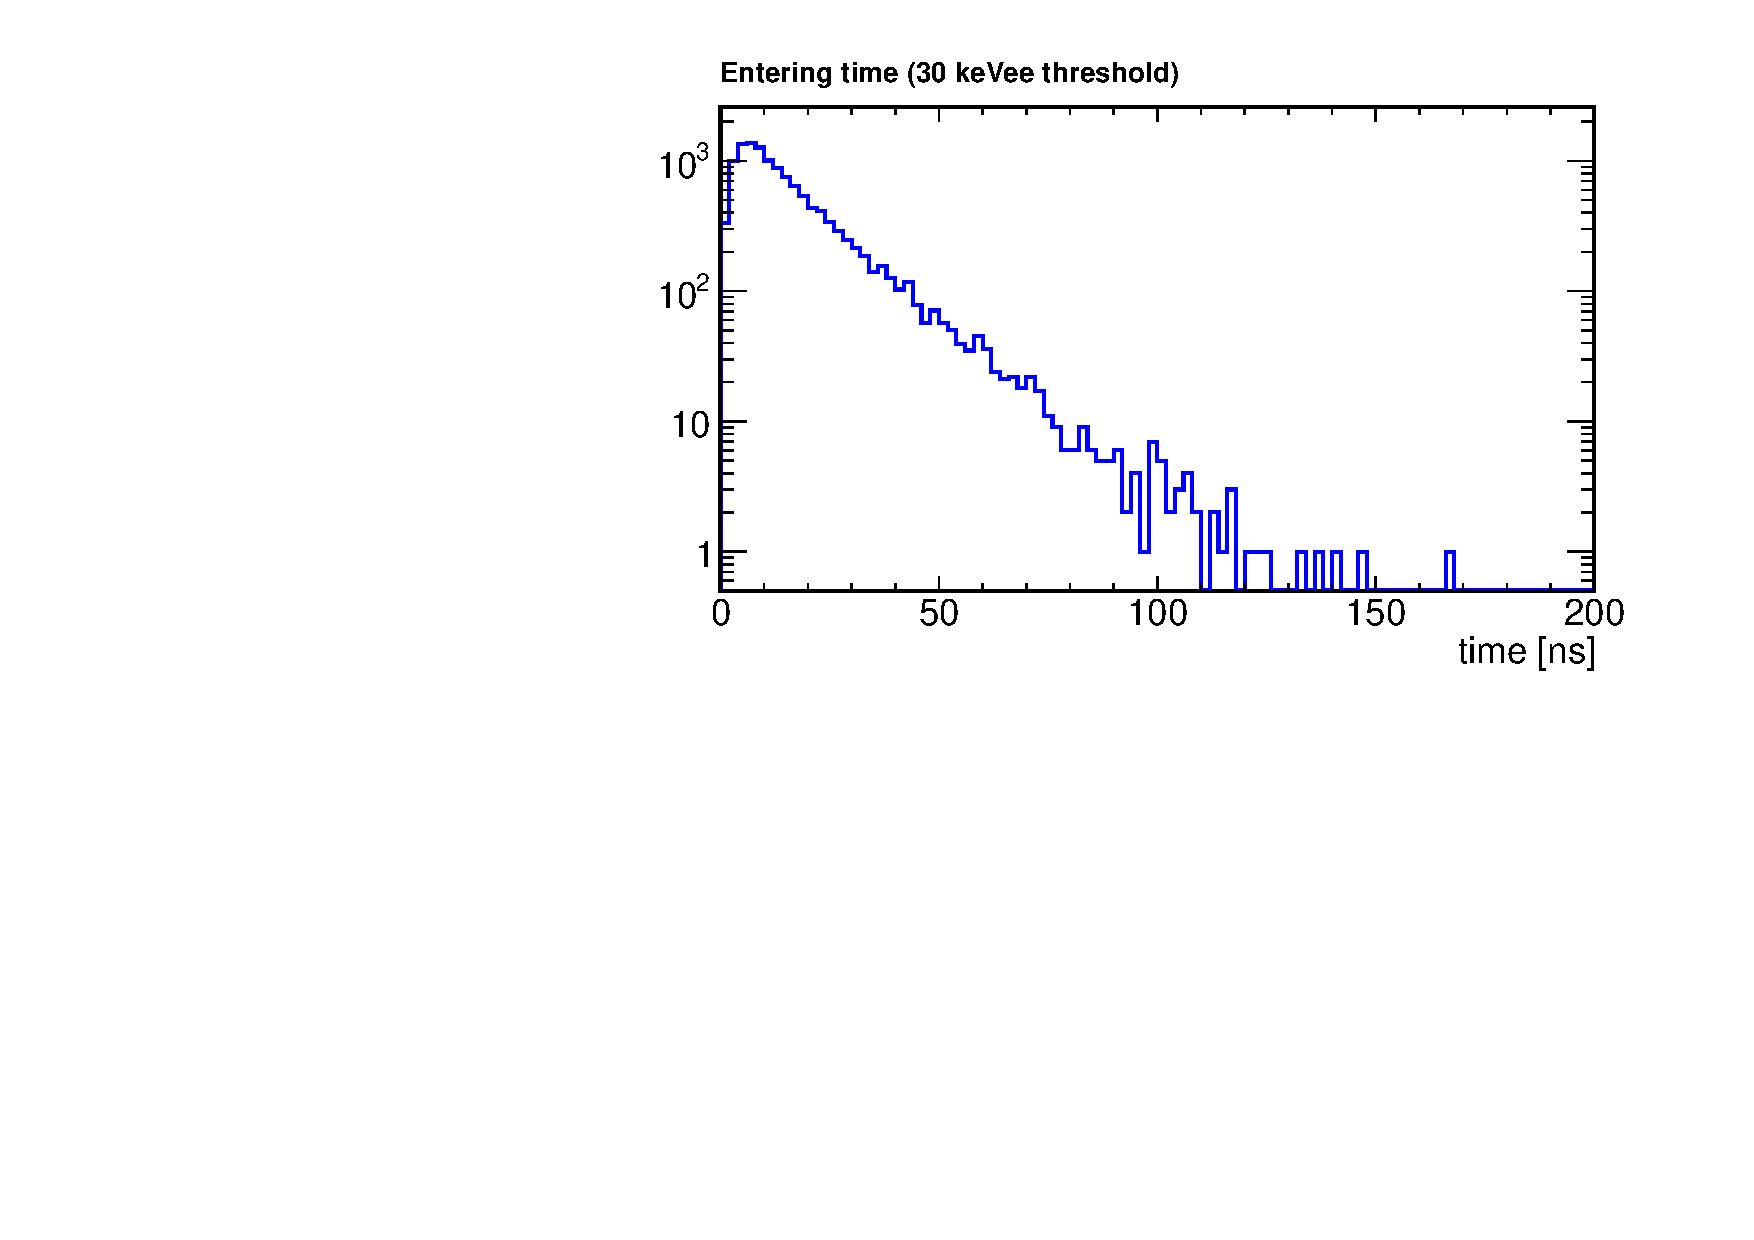
\includegraphics[trim = 0cm 0cm 0cm 1.1cm, clip, width=\textwidth]{pics/timing.pdf}
 	\caption{Blue curve: Geant4 simulation of $10^5$ neutrons; gray curve: MCNP simulation of unknown total number of primary neutrons.  Threshold is \SI{30}{keVee}.}
 	\label{fig:timing30}
 \end{figure}

The timing graphs of both, Geant4 and MCNP simulation, show a dropoff at \SI{0}{ns} due to the threshold and end somewhere between \SI{100}{ns} and \SI{150}{ns}.  

\subsection{Energy deposition}

Finally, the energy depositions of both simulations are being compared. Figure \ref{fig:photonResponse} provided the necessary data to convert the energy to electron equivalent (keVee). As mentioned before, $\gamma$ and $e^+$ are treated as $e^-$ and deuterons lie in the middle between $p$ and $\alpha$. Seldom particles like beryllium will be ignored.

Figure \ref{fig:edepFull} and \ref{fig:edepSmall} show the normalized count of valid events on a 60 day exposure. The blue curve uses the same photon response values as the MCNP code which was explained in paragraph \ref{part:eResponse}. The results of the MCNP simulation should look similar, but data was only available from 0-600 keVee (see black curve in fig. \ref{fig:edepSmall}). 
The red curve uses the photon response of fig \ref{fig:photonResponse} and is expected to be closer to the  data of the real detector. Both curves however, show a peak at 2.2 MeVee which is a result of neutron capture at hydrogen.
The green curve uses the same settings as the red one but a cutoff was applied after \SI{5}{\SIUnitSymbolMicro s}. This removes almost all 2.2 MeVee $\gamma$ from the neutron capture.

 \begin{figure}[H]
 	\centering
 		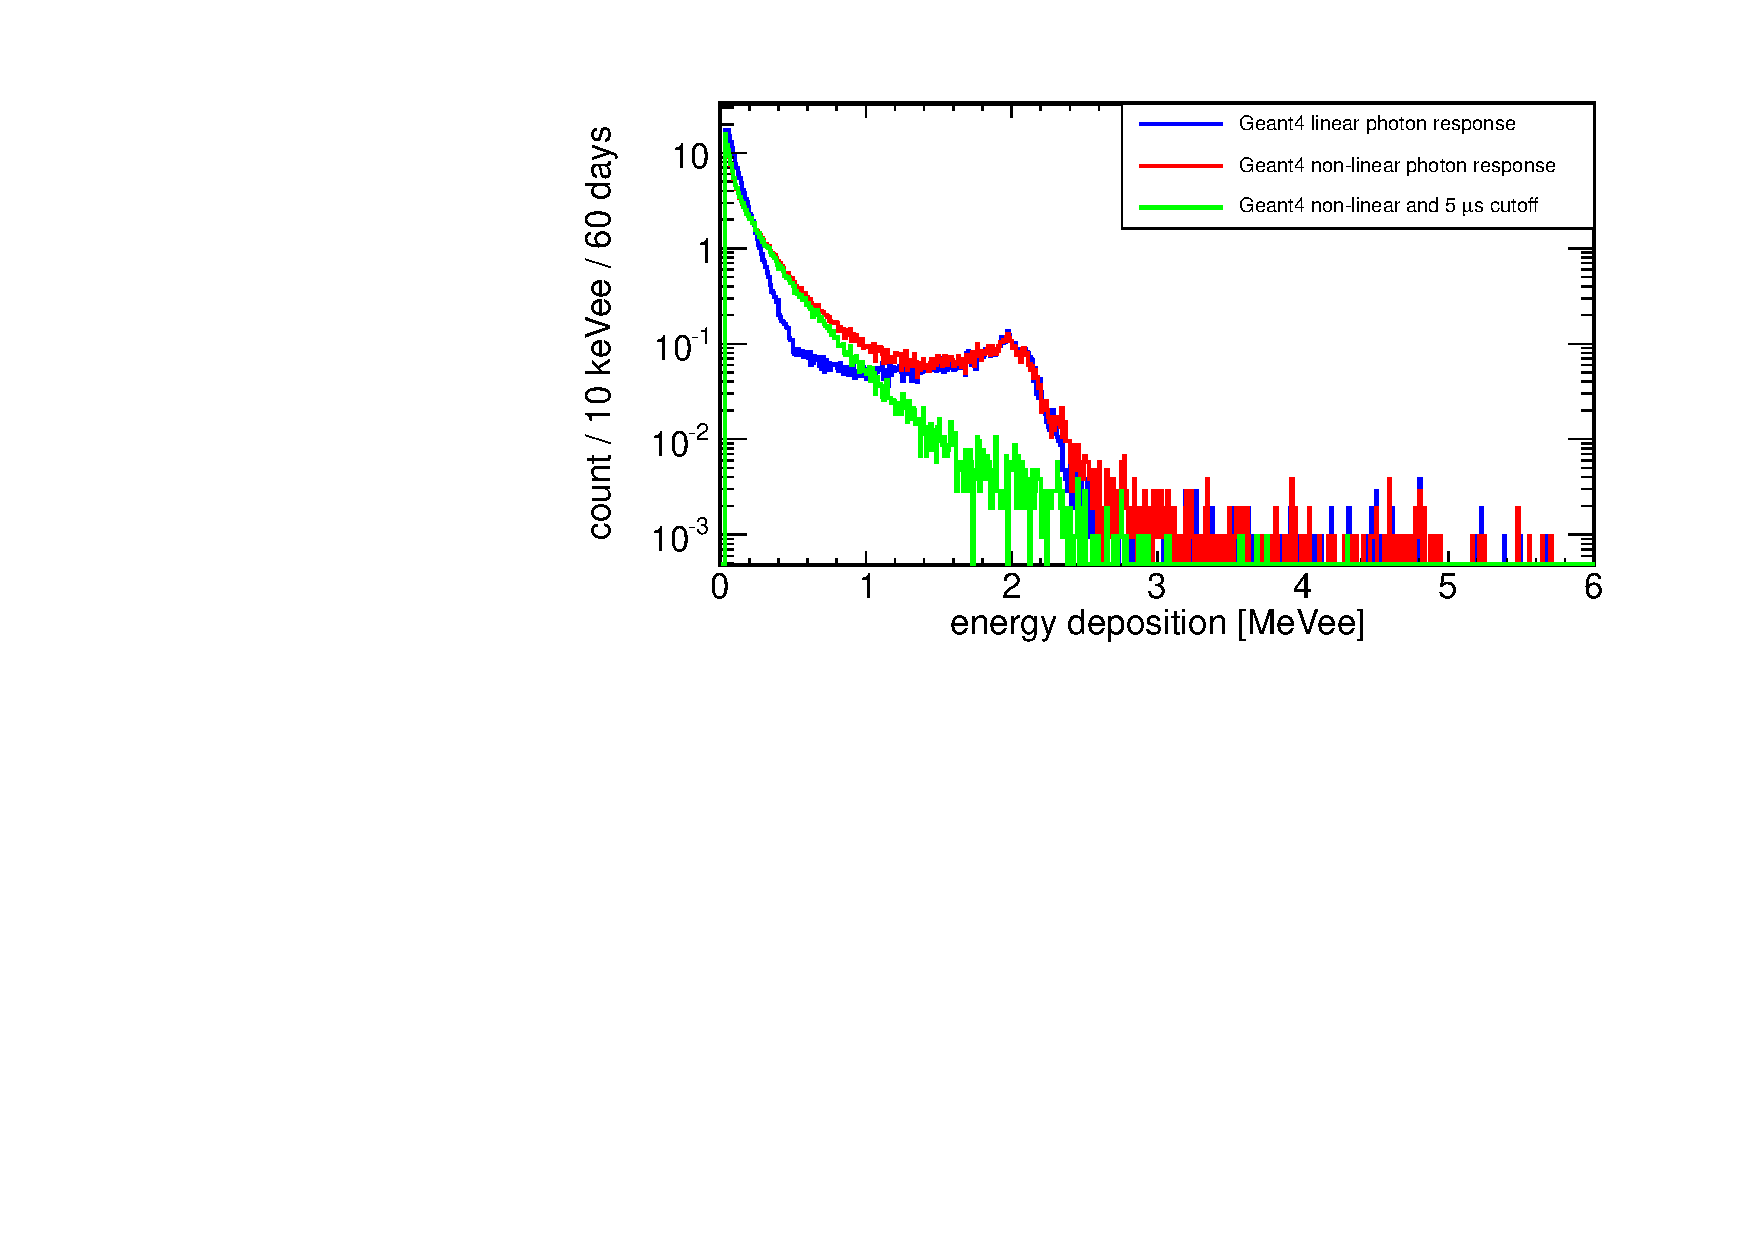
\includegraphics[width=1.\textwidth]{pics/edep_full.pdf}
 		\caption{Energy deposition of different energy settings in with Geant4. Blue curve uses the same settings as MCNP simulation and should resemble its results at energies $>$ \SI{600}{keVee}.}
 		\label{fig:edepFull}
\end{figure}
\begin{figure}[H]
	\centering
 		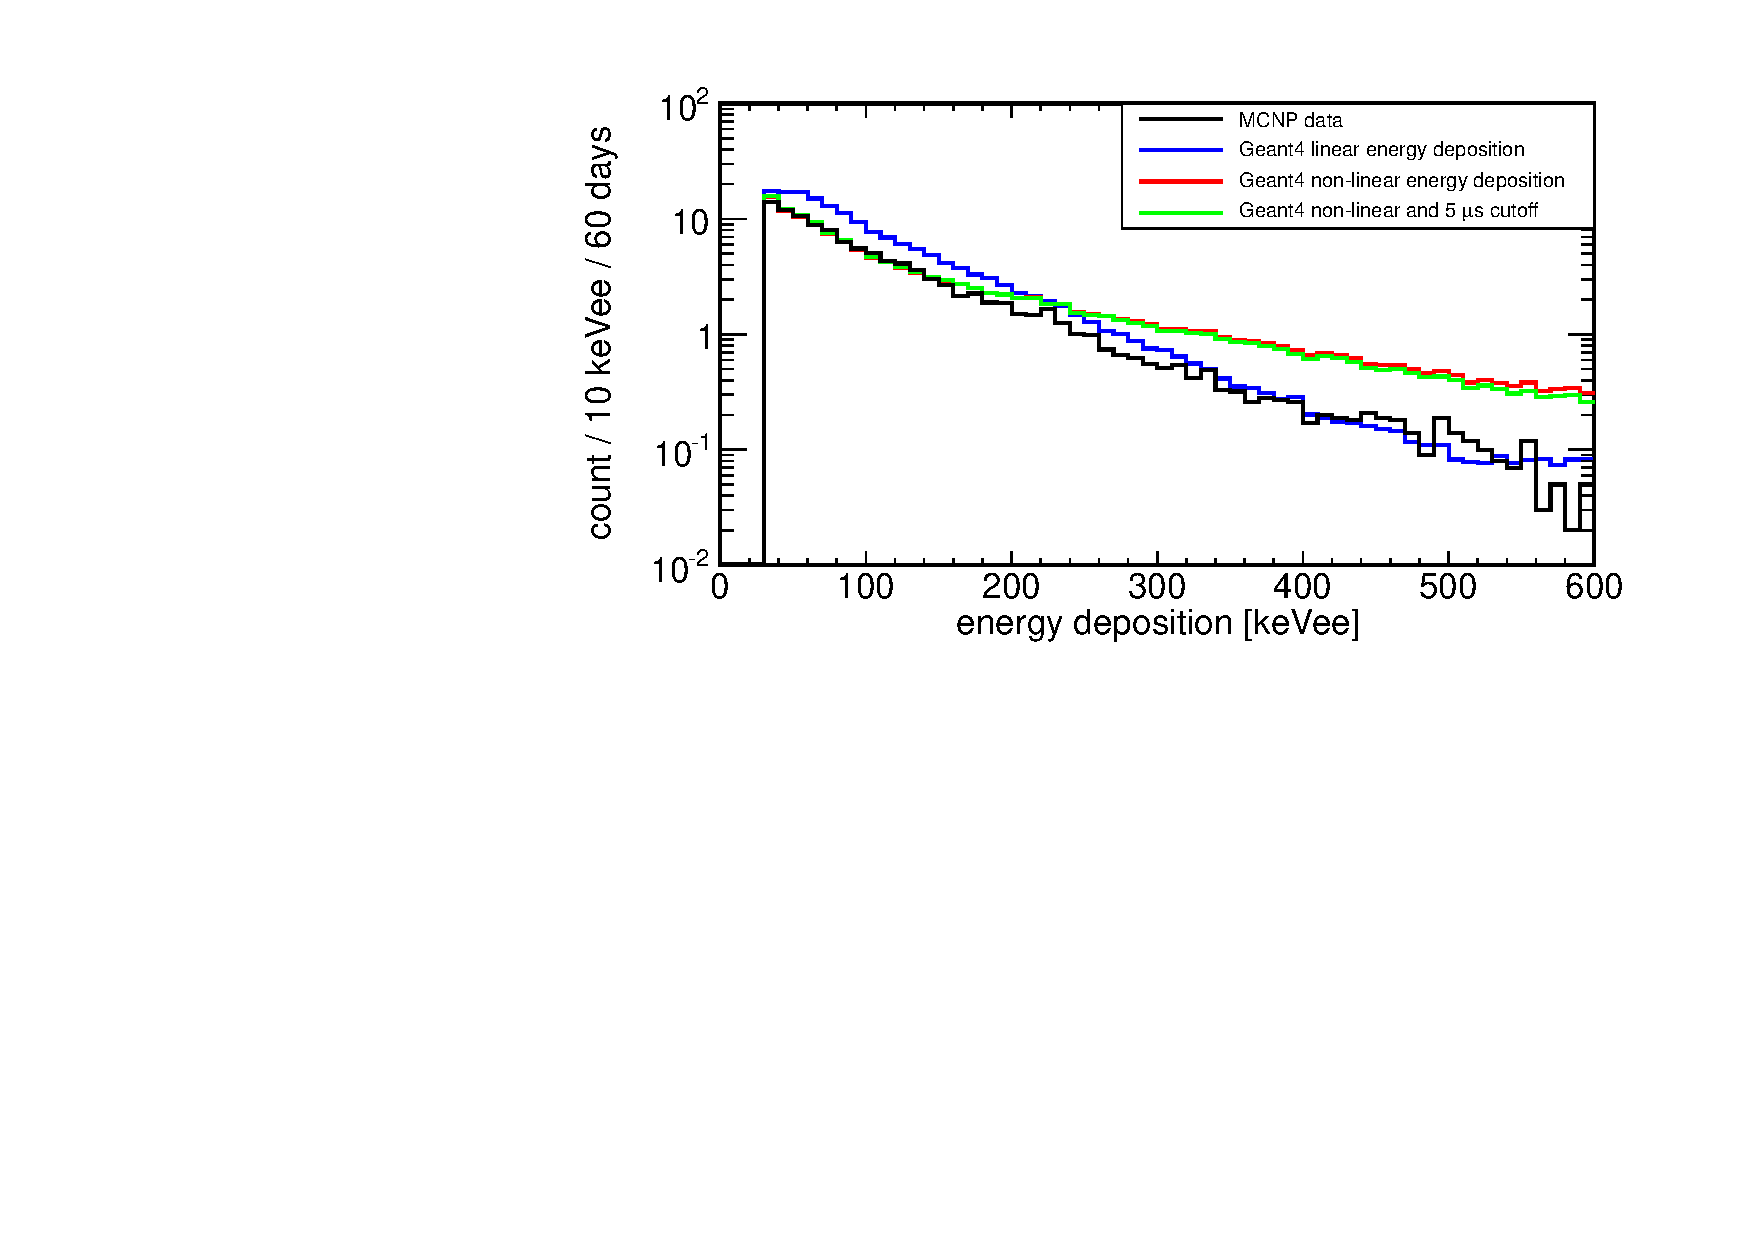
\includegraphics[width=1.\textwidth]{pics/edep_small.pdf}
 		\caption{Close up of figure \ref{fig:edepFull}. The black curve is the original data of the MCNP simulation that was only available from {0-600} {keVee}.}
 		\label{fig:edepSmall}
 	\end{figure} 
 	
 Figure \ref{fig:edepSmall} shows a closeup of figure \ref{fig:edepFull} from 0-600 keVee. The blue curve has the same slope as the original data (black) but there is a small offset in the beginning.
 The red and the green curve stay close together and even match the original data from 1-200 keVee better than the blue curve does but after that they sheer off from the original data.
 
 As can be seen in figure \ref{fig:edepFull} the blue curve shows a sharper drop off between 0.2 and 1.4 MeV than the red curve due to the linear energy deposition. Both curves have a peak at \SI{2.2}{MeVee} which is a result of neutron capture at hydrogen. This process emits a \SI{2.2}{MeVee} $\gamma$, that will deposit all of its energy in most events.
 
The only difference between the red and the green curve is the \SI{5}{\SIUnitSymbolMicro s} cutoff but the effect of this is almost neglitable for energies $<600 \text{ keVee}$ and the green curve is only a little bit below the red one.
 
\section{Conclusion}
It was possible to roughly reproduce the results of the MCNP simulation using the Geant4 framework to some point. The most significant difference is the higher efficiency of the detector that was simulated with Geant4 as can be seen in figure \ref{fig:efficiency30} and \ref{fig:efficiency100}. Also, signals are detected earlier (figure \ref{fig:timing30}). Both differences might be a result of a slightly different detector geometry. The lead in this simulation weights $\sim \SI{550}{kg}$ whereas the MCNP data uses \SI{660}{kg} lead \cite[p.1]{MCNP}. Both lead boxes have the same size which means that the missing material lies in the 4 scintillator-holes and the scintillators. These are most likely bigger in this simulation because their size was estimated from the sketch in figure \ref{fig:detector} since it does not show their exact size.

Nevertheless both curves in figure \ref{fig:efficiency30} and \ref{fig:efficiency100} have the same structure which means that the relevant physical processes are equivalent. Also, the curves in figure \ref{fig:timing30} and figure \ref{fig:edepSmall} (black and blue curve) match reasonably which indicates that a bigger scintillator does not have a high overall influence.

\section{Further investigation}
Under real conditions the physical processes that occur equation (\ref{eq:reaction}) can also emit two neutrons at once instead of a single one. 

 \begin{align}
  \nu_{e}\hspace{0.5em}&+\hspace{0.5em}^{208}Pb\hspace{0.5em}\rightarrow\hspace{0.5em}^{208}Bi^{*}\hspace{0.5em}+\hspace{0.5em}e^-\label{eq:reaction}\\ &\rightarrow 1n,\hspace{0.5em}\bf{2n}\hspace{0.5em}\text{emission}\nonumber\\\nonumber\\
  \nu_{x}\hspace{0.5em}&+\hspace{0.5em}^{208}Pb\hspace{0.5em}\rightarrow\hspace{0.5em}^{208}Pb^{*}\hspace{0.5em}+\hspace{0.5em}\nu_{x}\nonumber\\ &\rightarrow 1n,\hspace{0.5em}\bf{2n},\hspace{0.5em}\gamma\hspace{0.5em}\text{emission}\nonumber
 \end{align}
 This behavior was not studied in this simulation so far but was already implemented in the code. Using these settings the data should get a lot closer to the actual detector results. 


\section*{Acknowledgments}
\begin{itemize}
  \item[] I want to express my gratitude to Kate Scholberg and the Duke Neutrino Group who supported me throughout this project. It was fun and very exciting to work with you.
  \item[] I also thank DAAD and RISE for providing this summer internship to me.
\end{itemize}

\bibliographystyle{my_utphys}
\bibliography{Final}

\end{document}
